% !TEX root = main.tex

\section{Context and scope of the project}
\subsection{Context}

Nowadays one of the most extensive uses of computing is artificial intelligence. This is being
used from, based on our preferences, help us select what products we can buy to properly detect
and focus faces when taking a picture. The main advantage of this field is that it reduces the
amount of human intervention and it usually performs better.

Inside AI one of the domains that has greatly increased during the last years is 
\emph{Machine Learning}. The main advantage is that it can solely learn from examples without 
explicit teaching, and thus reducing the human interaction during the learning process. One of the 
most used types is \emph{deep neural networks} and these have demonstrated impressive performance 
against tasks like the classification of digits from the MNIST data set.
~\cites{MNIST}{empirical-evaluation-deep-architectures}

Regarding the medical field, recent deep learning algorithms, specially convolutional networks 
have started to push the boundaries of precision medicine. 
Traditionally, medical predictions have been based on a few clinical parameters with poor accuracy.
However, other data types are available to improve such predictions. In this context, medical
images generated from MRI, PET or CT scans are vastly underused due to the inability of radiologists
to quantitatively analyze this complex data.

Different methods have appeared to analyze these images for tasks such as
image classification, object detection, segmentation and registration among other tasks. This
approach started in the late 1990s and has slowly shifted from systems that are completely designed
by humans to systems that are trained by computers using example data. 
~\cite{survey-deep-learning}

Professor Benjamin Haibe-Kains has helped in the development of \emph{Radiomics}, a new field to
relying on pre-defined, hand-engineered features computed from medical images to better 
characterize tumours and predict survival outcome. Although promising, radiomics suffers from 
two several limitations: the number of features is limited and it is a slow process as it requires
a radiologist to manually contour the tumour. Deep learning has the potential to address both issues
by automatically extract more information from the images.
~\cite{radiomics-ML-classifiers}

\subsubsection{Survival Analysis}

To use all this data, Survival Prediction models have been created. Data from these models have
three elements: a patient's baseline data \( x \), a failure event time 
\( T \), and an event indicator \( E \). If an event (e.g. death) is observed, the time 
interval \( T \) corresponds to the time elapsed between the time in which the \( x \)
data was collected and event's time, and the event indicator is \( E = 1 \). If an
event is not observed, the time interval \( T \) corresponds to the time elapsed between
the collection of the baseline data and the last contact with the patient, and the 
event indicator is \( E = 0 \). In this case, the patient is said to be
\emph{right-censored}.
~\cite{DeepSurv}

The survival and hazard functions are the two fundamental functions in survival analysis. The
survival function \( S(t) = \Pr(T \ge t) \), is the probability that an individual has
\emph{survived} beyond time \( t \). The hazard function \( \lambda(t) \) is a measure of risk at 
time \( t \) and it's defined as:
~\cite{Cox}
\[
  \lambda(t) = \lim_{\Delta t \rightarrow 0}
  \frac{\Pr(t \le T < t + \Delta t | T \ge t)}{\Delta t}
\]

Casting the survival analysis as a ranking problem is a way of dealing with the biased
distributions of survival times and the censoring data. Two subjects' survival times can be 
ordered only if:
\begin{enumerate}[noitemsep, topsep=0pt]
  \item Both of them are uncensored (\( E_i = E_j = 0\))
  \item The uncensored time of one is smaller than the censored survival time of the other
  (\( T_i < T_j | E_i = 1; E_j = 0 \))
\end{enumerate}

This can be visualized by means of an order graph \( G = (V, E) \), see \autoref{fig:graph}.
The set of vertices \( V \) represents all the individuals, where each filled vertex indicates
an \emph{uncensored} survival time, while an empty circle denotes a \emph{censored} observation.
Existence of an edge \( E_{ij} \) implies that \( T_i < T_j \). An edge cannot originate 
from a censored point.

\begin{figure}
  \centering
  \begin{subfigure}[b]{.4\textwidth}
    \centering
    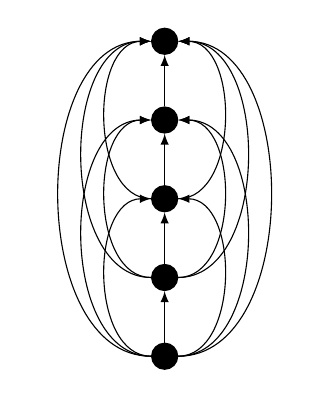
\begin{tikzpicture}
  \tikzstyle{bDot}=[circle, fill=black, draw]
  \foreach \y in {1,...,5} {
    \node[bDot] (D-\y) at (0, \y) {};
  }

  \foreach \y in {1,...,4} {
    \pgfmathsetmacro{\z}{int(\y + 1)}
    \draw[-latex] (D-\y) -- ({D-\z}.south);
  }

  \foreach \y in {1,...,3} {
    \pgfmathsetmacro{\z}{int(\y + 2)}
    \foreach \j in {\z,...,5} {
      \ifthenelse{\y=2 \OR \y=3}{
        \draw[-latex] (D-\y) to[bend left=90] (D-\j);
      }{
        \draw[-latex] (D-\y) to[bend right=90] (D-\j);
      }
    }
  }
\end{tikzpicture}

    \caption{No censored data}
  \end{subfigure}
  ~
  \begin{subfigure}[b]{.4\textwidth}
    \centering
    \begin{tikzpicture}
  \foreach \y in {1,...,5} {
    \ifthenelse{\y=2 \OR \y=4}{
      \node [circle, fill=white, draw=black] (D-\y) at (0, \y) {};
    }{
      \node [circle, fill=black, draw=black] (D-\y) at (0, \y) {};
    }

    \foreach \y in {3,4,5} {
      \draw [-latex] (D-1) to[bend right=90] (D-\y);
    }

    \foreach \y/\z in {1/2, 3/4} {
      \draw [-latex] (D-\y) -- (D-\z);
    }
    \draw [-latex] (D-3) to[bend left=90] (D-5);
  }
\end{tikzpicture}

    \caption{Censored data}
  \end{subfigure}

  \caption{Order graphs representing the ranking constraints \label{fig:graph}}
\end{figure}

% C-index explanation
The standard performance measure, to compare if a survival 
model is performing better than another, is the \emph{Concordance Index} (C-index). This 
index is 1 for a perfect data fit and 0.5 for a random model. Also, another comparison 
element is the ROC curve which represents the \emph{False Positive Rate} against the 
\emph{True Positive Rate}, see \autoref{fig:ROC-curve}. Usually the C-index is seen as 
the area under the ROC curve.
~\cites{ROC-precision-recall}{RankingCI}

\begin{figure}
  \centering
  \includegraphics[width=.5\linewidth]{images/roc_curve}
  \caption{ROC Curve example\label{fig:ROC-curve}}
\end{figure}

\subsection{Problem Formulation}

Through a collaboration with Dr.~Fei-Fei Liu, head of the Radiation Medicine Program at Princess
Margaret Cancer Centre, prof. Benjamin Haibe-Kains has access to a unique set of \( {\sim}500 \) 
scans of head-and-neck cancer patients with associated survival data. 

The goal of this project is to develop a new deep learning model to analyze this private 
dataset in combination with public databases to improve the prediction rate of patients' 
survival compared to models built on traditional radiomic features. The model should be 
able to get better results than the ones obtained using the radiomic \texttt{VOLUME} feature
which usually achieves a C-index of 0.65. The developed model should try to improve this value.

\subsection{State-of-the-art}

Nowadays, a lot of research is being done in the medical field using deep learning. Image
classification is one of the first areas in which there's a major contribution to medical analysis.
Usually in image classification one has one or multiple images as input and a single diagnostic 
variable as output (e.g.~ill or not). With this approach the use of transfer learning has been a
great improvement.
~\cite{survey-deep-learning}

Transfer learning is the use of pre-trained networks to reduce the requirement of large data
sets for deep network training. Usually, there are two possible strategies: 
\begin{itemize}[noitemsep, topsep=0pt]
  \item Using a pre-trained NN as a feature extractor
  \item Fine-tuning a pre-trained network on medical data.
\end{itemize}

Both strategies are popular and have been widely applied. One of the networks that allow this type
of retrain is GoogLeNet Inception v3.
~\cites{GoogLeNet}{NNRetrain}{inceptionRetrain}

Moreover, regarding the prediction of survival models there have been different approaches but
almost all of them use MRI, PET or CT scans and the clinical data. The typical one is to extract
hand-crafted radiomic features using own methods or using libraries such as
\href{https://github.com/Radiomics/pyradiomics}{\emph{PyRadiomics}}. This hand-crafted features are
based in things like tumour shape intensity, shape, volume or texture.
~\cites{PyRadiomics}{tumour-radiomics}

The other approach, is using a deep learning-based model for prediction. In this case too, 
hand-crafted features are extracted but, a Convolutional Neural Network is used to extract
features instead. So, this way, the number of extracted features is bigger. However,
there's the additional problem that usually medical imaging data is 3D but, when working 
with CNN, only 2D images can be used, since there is still no pre-trained CNN on 3D images.
Although this method seems promising still requires further work to train a dedicated 
feature extractor explicitly designed for medical images.
~\cite{deep-learning-radiomics-gbm}

An implemented survival prediction model is \emph{DeepSurv} which is based on survival data
and uses the Cox Proportional Hazards model an individual's survival given the baseline data
\( x \). It's an Open Source Python module that applies recent deep learning techniques 
to the Cox model.
~\cites{DeepSurv}{Cox}

\subsection{Stakeholders}



\subsection{Scope}

The first task will be learning and understanding how Neural Networks and specifically how 
Convolutional Neural Networks Work. This way I will have a fully understanding of the background
that all this methods use create models for survival prediction.

The next task will be setting up and running the \emph{DeepSurv} python package on a local 
computer. This will mean trying to test all the methods that can be used and see which parts 
can be reused to create a new Survival Prediction Model. Since this model is not prepared
to have images as input, an improvement will be to add the possibility to pass medical 
images as input to train the survival model. 

Afterwards a deep learning model will be created starting from zero but trying to reuse
as many parts as possible. This model will not be using Cox Proportional Hazards but instead
it will be created using a Siamese Network. This type of networks are useful for comparison
tasks such as face recognition. 

\subsection{Methodology}

This project is part of a research project at Benjamin Haibe-Kains Bioinformatics and 
Computational Genomics Laboratory. This means that every week there will be a laboratory meeting
where progress will be presented to all the lab members and feedback will be received accordingly. 

Also since there are different ways of development this means that it will have a process of trial
and error until the proper solution is found. This means that during this process the
tasks will be assigned on a weekly basis.
